\documentclass[final,t]{beamer}
\mode<presentation>
 {
  \usetheme{boxes}
 }

\usepackage[orientation=landscape,size=a1,scale=1.3,debug]{beamerposter}
\usepackage{wrapfig}
\usepackage{background}
\usepackage{lipsum} % for dummy text
\usepackage{tcolorbox}
% \usepackage{helvet}
\usepackage{svg}
% \renewcommand{\familydefault}{\sfdefault}
\usepackage{fontspec}
\setsansfont{Avenir LT Std}
\usebackgroundtemplate{\includesvg[width=\paperwidth]{template}}%
\tcbuselibrary{skins}


\title[]{\Huge\bfseries Syringe Pump for Electrochemical Cell}
\author[]{\large \textbf{Dolica Akello-Egwel} \and Gary Yendell \\ 2018 Cohort / Mantid Team}
\date{}

% Remove Beamer Navigation Symbols
\setbeamercolor*{frametitle}{bg=}
\setbeamertemplate{navigation symbols}{}

\begin{document}

\newtcolorbox{custombox}[1]
{
  % colback=blue!10!lightgray!35!white,
  colback=white,
  arc=1mm,
  % boxsep=5mm,
  colframe=blue!70!black,
  top=3mm,
  toptitle=3mm,
  bottomtitle=3mm,
  fonttitle=\large\bfseries,
  coltitle=white,
  title=#1,
  % parbox=false,
}

\AfterEndEnvironment{custombox}{\vspace{0.6cm}}
\AfterEndEnvironment{figure}{\vspace{0.6cm}}

\begin{frame}
\maketitle
\begin{columns}[t]
  \begin{column}{.32\linewidth}
 
  \begin{custombox}{Introduction}
      The existing streamDevice-based EPICS driver for the Hamilton Microlab 500/600 Syringe Pump was not
      especially suited to sending "complex" commands that contain two or more instructions.
      The driver also lacked the ability to reliably send simultaneous commands to both syringes, and to
      cycle sets of simultaneous commands indefinetly. The aim of this project was to create a user-friendly
      and extensible Python API that allows users to easily create continuous flows through an electrochemical
      cell.
  \end{custombox}

  \begin{custombox}{Objectives}
     \begin{itemize}
        \item Make a Python library for controlling the Hamilton Microlab Syringe Pump 
        \item Add EDM screens 
        \item Add a cycling ability to allow 
        \item Interface with EPICS. 
    \end{itemize} 
  \end{custombox}

      \begin{figure}[t]
          {%
        \setlength{\fboxsep}{0pt}%
        \setlength{\fboxrule}{3pt}%
          \fbox{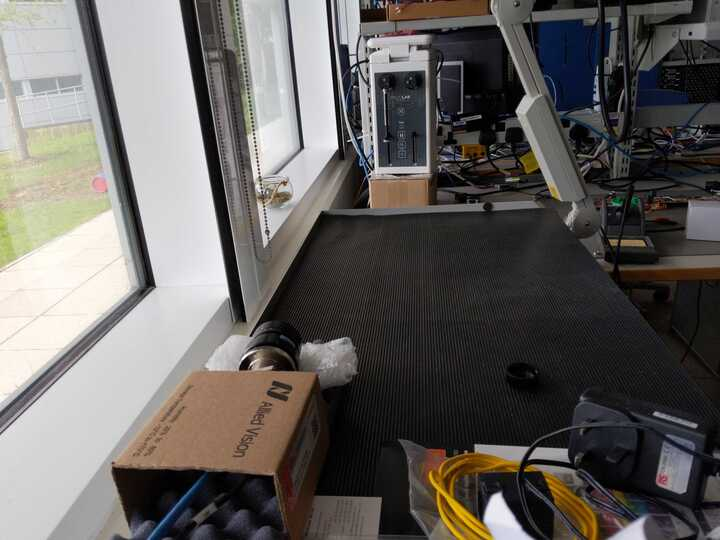
\includegraphics[width=0.7\linewidth]{images/camerasetup}}%
        }%
% \centering
      \end{figure}

  \end{column}

 %%%%%%%%%%%%%%%%%%%%%%%%%%%%%%%%%%%%%%%%%%%%%%%%%%%%%%%%%%%


  \begin{column}{.32\linewidth}

  \begin{custombox}{Implementation}
    Discuss the Python library. 
  \end{custombox}
  
      \begin{figure}[t]
          {%
        \setlength{\fboxsep}{0pt}%
        \setlength{\fboxrule}{3pt}%
          \fbox{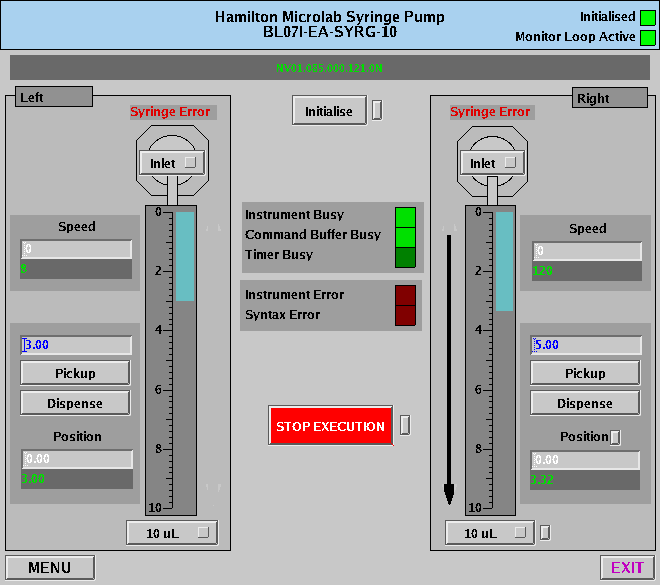
\includegraphics[width=0.8\linewidth]{images/mainscreen.png}}%
              \caption{EDM screen}
        }%
% \centering
\end{figure}

  \end{column}

  
  %%%%%%%%%%%%%%%%%%%%%%%%%%%%%%%%%%%%%%%%%%%%%%%%%%%%%%%%%%%

  \begin{column}{.32\linewidth}

      \begin{custombox}{EPICS and \texttt{softioc}}
          \begin{wrapfigure}{r}{0.3\textwidth}
      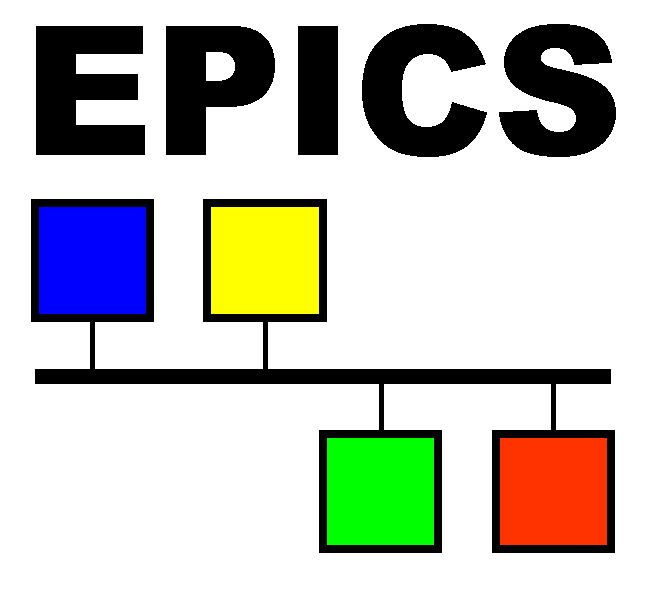
\includegraphics[width=\linewidth]{images/epicslogo}
          \end{wrapfigure}
      The Experimental Physics and Industrial Control System (EPICS) comprises a set of software components and
      tools that can be used to create distributed control systems. EPICS provides capabilities that are typically expected from a distributed control system:
  \end{custombox}

 
  \begin{custombox}{Results}
    \begin{itemize}
        \item Permanent "Syringe Error" message 
        \item Behaviour of syringe movement indicator arrows not ideal, especially for fast movements 
    \end{itemize}
  \end{custombox}

  \begin{custombox}{Further Work}
    \begin{itemize}
        \item Develop a simulator for the syringe pump and use it to create system tests
        \item Add a cleaning command 
    \end{itemize}
  \end{custombox}
  \end{column}
  \end{columns}
    
\end{frame}

\end{document}
